\documentclass[a4paper,11pt,onecolumn,oneside,UTF8]{article}

\usepackage{ctex}     % 中文支持
\usepackage{amsthm,amsmath,amssymb}
\usepackage{mathrsfs}
\usepackage{bm}       % 公式中的粗体字符(用命令\boldsymbol)
\usepackage{graphicx, subfig}
\usepackage{caption}
\usepackage{float}
\usepackage{color}
\usepackage{enumerate}
\usepackage{multirow}
\usepackage{pgfplots}
\usepackage{tikz}
\usepackage{listings}
\usepackage[colorlinks,linkcolor=blue]{hyperref}

\addtolength{\topmargin}{-54pt}
\setlength{\oddsidemargin}{-0.9cm}  % 3.17cm - 1 inch
\setlength{\evensidemargin}{\oddsidemargin}
\setlength{\textwidth}{18.00cm}
\setlength{\textheight}{24.00cm}    % 24.62
\lstset{
 columns=fixed,       
 frame=none,                                          % 不显示背景边框
 backgroundcolor=\color[RGB]{245,245,244},            % 设定背景颜色
 numberstyle=\footnotesize\color{darkgray},           % 设置数字样式
 commentstyle=\it\color[RGB]{0,96,96},                % 设置代码注释的格式
 stringstyle=\rmfamily\slshape\color[RGB]{128,0,0},   % 设置字符串格式
 showstringspaces=false,                              % 不显示字符串中的空格
%  language=bash,                                       % 设置语言
%  numbers=left,                                        % 在左侧显示行号
%  numberstyle=\tiny\color{gray},                       % 设定行号格式
%  keywordstyle=\color[RGB]{40,40,255},                 % 设定关键字颜色
}

\begin{document}

\begin{center}
    \Large\textbf{Answer of Assignment 6\\PCA \& SVM}
\end{center}

\begin{flushright}
    2020E8017782032\_蒲尧
\end{flushright}

\section*{第一部分:计算与证明}

\begin{enumerate}
    \item 有$N$个样本$x_1,…, x_N$,每个样本维数$D$,希望将样本维数降低到$K$,请给出 PCA 算法的计算过程。
    \item 根据自己的理解简述结构风险最小化与 VC 维。
    \item 请推导出 Hard-Margin SVM 的优化目标。
    \item 请解释出 Hinge Loss 在 SVM 中的意义。
    \item 简述核方法的基本原理。
\end{enumerate}

\section*{第二部分: 计算机编程}
\begin{enumerate}[6.]
    \item 从MNIST数据集中任意选择两类,对其进行SVM分类,
          可调用现有的SVM工具如LIBSVM,展示超参数C以及核函数参数的选择过程。
\end{enumerate}


\section*{第一部分回答}

\begin{enumerate}
    \item
          PCA 算法的计算过程:\\
          \begin{enumerate}[(1)]
              \item 计算数据的均值:$\bar{\boldsymbol{x}} = \frac{1}{N}\sum \limits_{n=1}^N\boldsymbol{x}_n$;
              \item 计算样本的协方差矩阵:$\mathbf{S}=\sum \limits_{n=1}^N\left(x_n-\bar x\right)\left(x_n-\bar x\right)^T$;
              \item 做 D×D 维矩阵 $\mathbf{S}$ 的特征值分解;
              \item 提取其中最大的 K 个特征值对应的最大的 K 个特征向量 $\vec{u}_1,...,\vec{u}_K,\left(s.t. \lambda_1 \geq \lambda_2 \geq ...\geq \lambda_{K-1} \geq \lambda_{K} \geq \right)$,
                    得到 D×K 大小的映射矩阵 $\mathbf{U} = \left[\vec{u}_1,\vec{u}_2,...,\vec{u}_K\right]$;
              \item 将每个样本进行映射:$\boldsymbol{z}_n = \mathbf{U}^T\boldsymbol{x}_n$,得到的$\boldsymbol{z}_n$是 K×1 的向量。
          \end{enumerate}
    \item
          \begin{enumerate}[(1)]
              \item 结构风险最小化:在未知的测试集上的错误率达到最小化。$Test\ error\ rate <= train\ error\ rate + f(N, h, p)$
              \item VC维:某个空间中给n个样本点随机打标签,如果某个模型足够强大能够将其分开,则增加样本个数为n+1,直到不能分开n+1,则这个最大的样本点数n为该空间的VC维。
          \end{enumerate}
    \item
          Hard-Margin SVM 的优化目标\\
          点$\vec{x_i}$到直线$\vec{w}\vec{x}+\vec{b}=0$的距离为:
          $$
              \begin{aligned}
                  d\left(\vec{x_i}\right) = \frac{|\vec{w}\vec{x_i}+\vec{b}|}{\sqrt{||\vec{w}||_2^2}} \\
                  \left\{\begin{array}{ll}
                      \vec{w}\vec{x_i}+\vec{b}\geq 0, & y_i=1; \\
                      \vec{w}\vec{x_i}+\vec{b}\leq 0, & y_i=-1
                  \end{array}
                  \right.
              \end{aligned}
          $$
          我们的目标是最大化到直线最近点的距离 d,从而推出参数 $\vec{w},\vec{b}$:
          $$
              \begin{aligned}
                    & \max\limits_{\vec{w},\vec{b}}\min\limits_{\vec{x_i}\in\mathbf{D}} d                                                         \\
                  = & \max\limits_{\vec{w},\vec{b}}\min\limits_{\vec{x_i}\in\mathbf{D}} \frac{|\vec{w}\vec{x_i}+\vec{b}|}{\sqrt{||\vec{w}||_2^2}} \\
                    & s.t.\ \forall \vec{x_i}\in\mathbf{D}:\ y_i\left(\vec{w}\vec{x}+\vec{b}\right)\geq 0                                         \\
              \end{aligned}
          $$
          我们采用如下策略:
          $$
              \forall \vec{x_i}\in\mathbf{D}:\ |\vec{w}\vec{x}+\vec{b}|\geq 1
          $$
          我们可以推出:
          $$
              \min\limits_{\vec{x_i}\in\mathbf{D}} \frac{|\vec{w}\vec{x_i}+\vec{b}|}{\sqrt{||\vec{w}||_2^2}}\geq \min\limits_{\vec{x_i}\in\mathbf{D}} \frac{1}{\sqrt{||\vec{w}||_2^2}} = \frac{1}{\sqrt{||\vec{w}||_2^2}} = \frac{1}{||\vec{w}||}
          $$
          直线两侧都有点,距离×2,得到最终优化目标:
          $$
              \max \frac{2}{||\vec{w}||}
          $$
    \item
          对于Soft-margin SVM,优化目标可以写成:
          $$
              \min\limits_{\vec{w},b}\frac{||\vec{w}||^2}{2}+C\sum\limits_{i=1}^m \mathscr{L}_{0/1}\left(y_i\left(\vec{w}^T\vec{x}_i+b\right)-1\right)
          $$
          其中,C>0 是一个常数,作为惩罚因子,$\mathscr{L}_{0/1}$ 是“0/1损失函数”:
          $$
              \mathscr{L}_{0/1}\left(z\right) = \left\{\begin{array}{ll}
                  1, & \text{if }z<0;   \\
                  0, & \text{otherwise}
              \end{array}
              \right.
          $$
          Hinge Loss:
          $$
              \mathscr{L}_{hinge}\left(z\right) = \max\left(0,1-z\right)
          $$
          Hinge Loss 的零区域对应的正是非支持向量的普通样本,从而所有的普通样本都不参与最终超平面的决定;只考虑支持向量。这正是支持向量机最大的优势所在,对训练样本数目的依赖大大减少,从而且提高了训练效率。
    \item
          核方法:回顾前面得到的公式:
          $$
              \begin{aligned}
                  \max \sum \limits_{i=1}^n\alpha_i-\frac{1}{2}\sum\limits_{i=1,j=1}^n\alpha_i\alpha_jy_iy_jx_ix_j \\
                  s.t.\ C\geq\alpha_i\geq 0,\ \sum\limits_{i=1}^n\alpha_iy_i=0
              \end{aligned}
          $$
          我们看到计算目标函数时,需要知道x的内积。我们引入核函数,一个可以应用于一对输入数据以计算对应特征空间中的内积的函数。对于不能线性分割的数据集,核函数可以将数据升高维度,进行高纬度的内积,寻找高纬度数据的相似性和高纬度的线性分界面。
\end{enumerate}

\section*{第二部分回答}

代码见如下文件
\href{https://github.com/Allenem/PatternRecognition/blob/main/hw6/hw6.py}{Python文件}。
由图可知:C过小,欠拟合,准确度较小;C过大,过拟合,Test和Train的准确率相差会变大。gamma过小准确度较小,gamma越大准确度相对变大。\\
\begin{figure}[H]
    \centering
    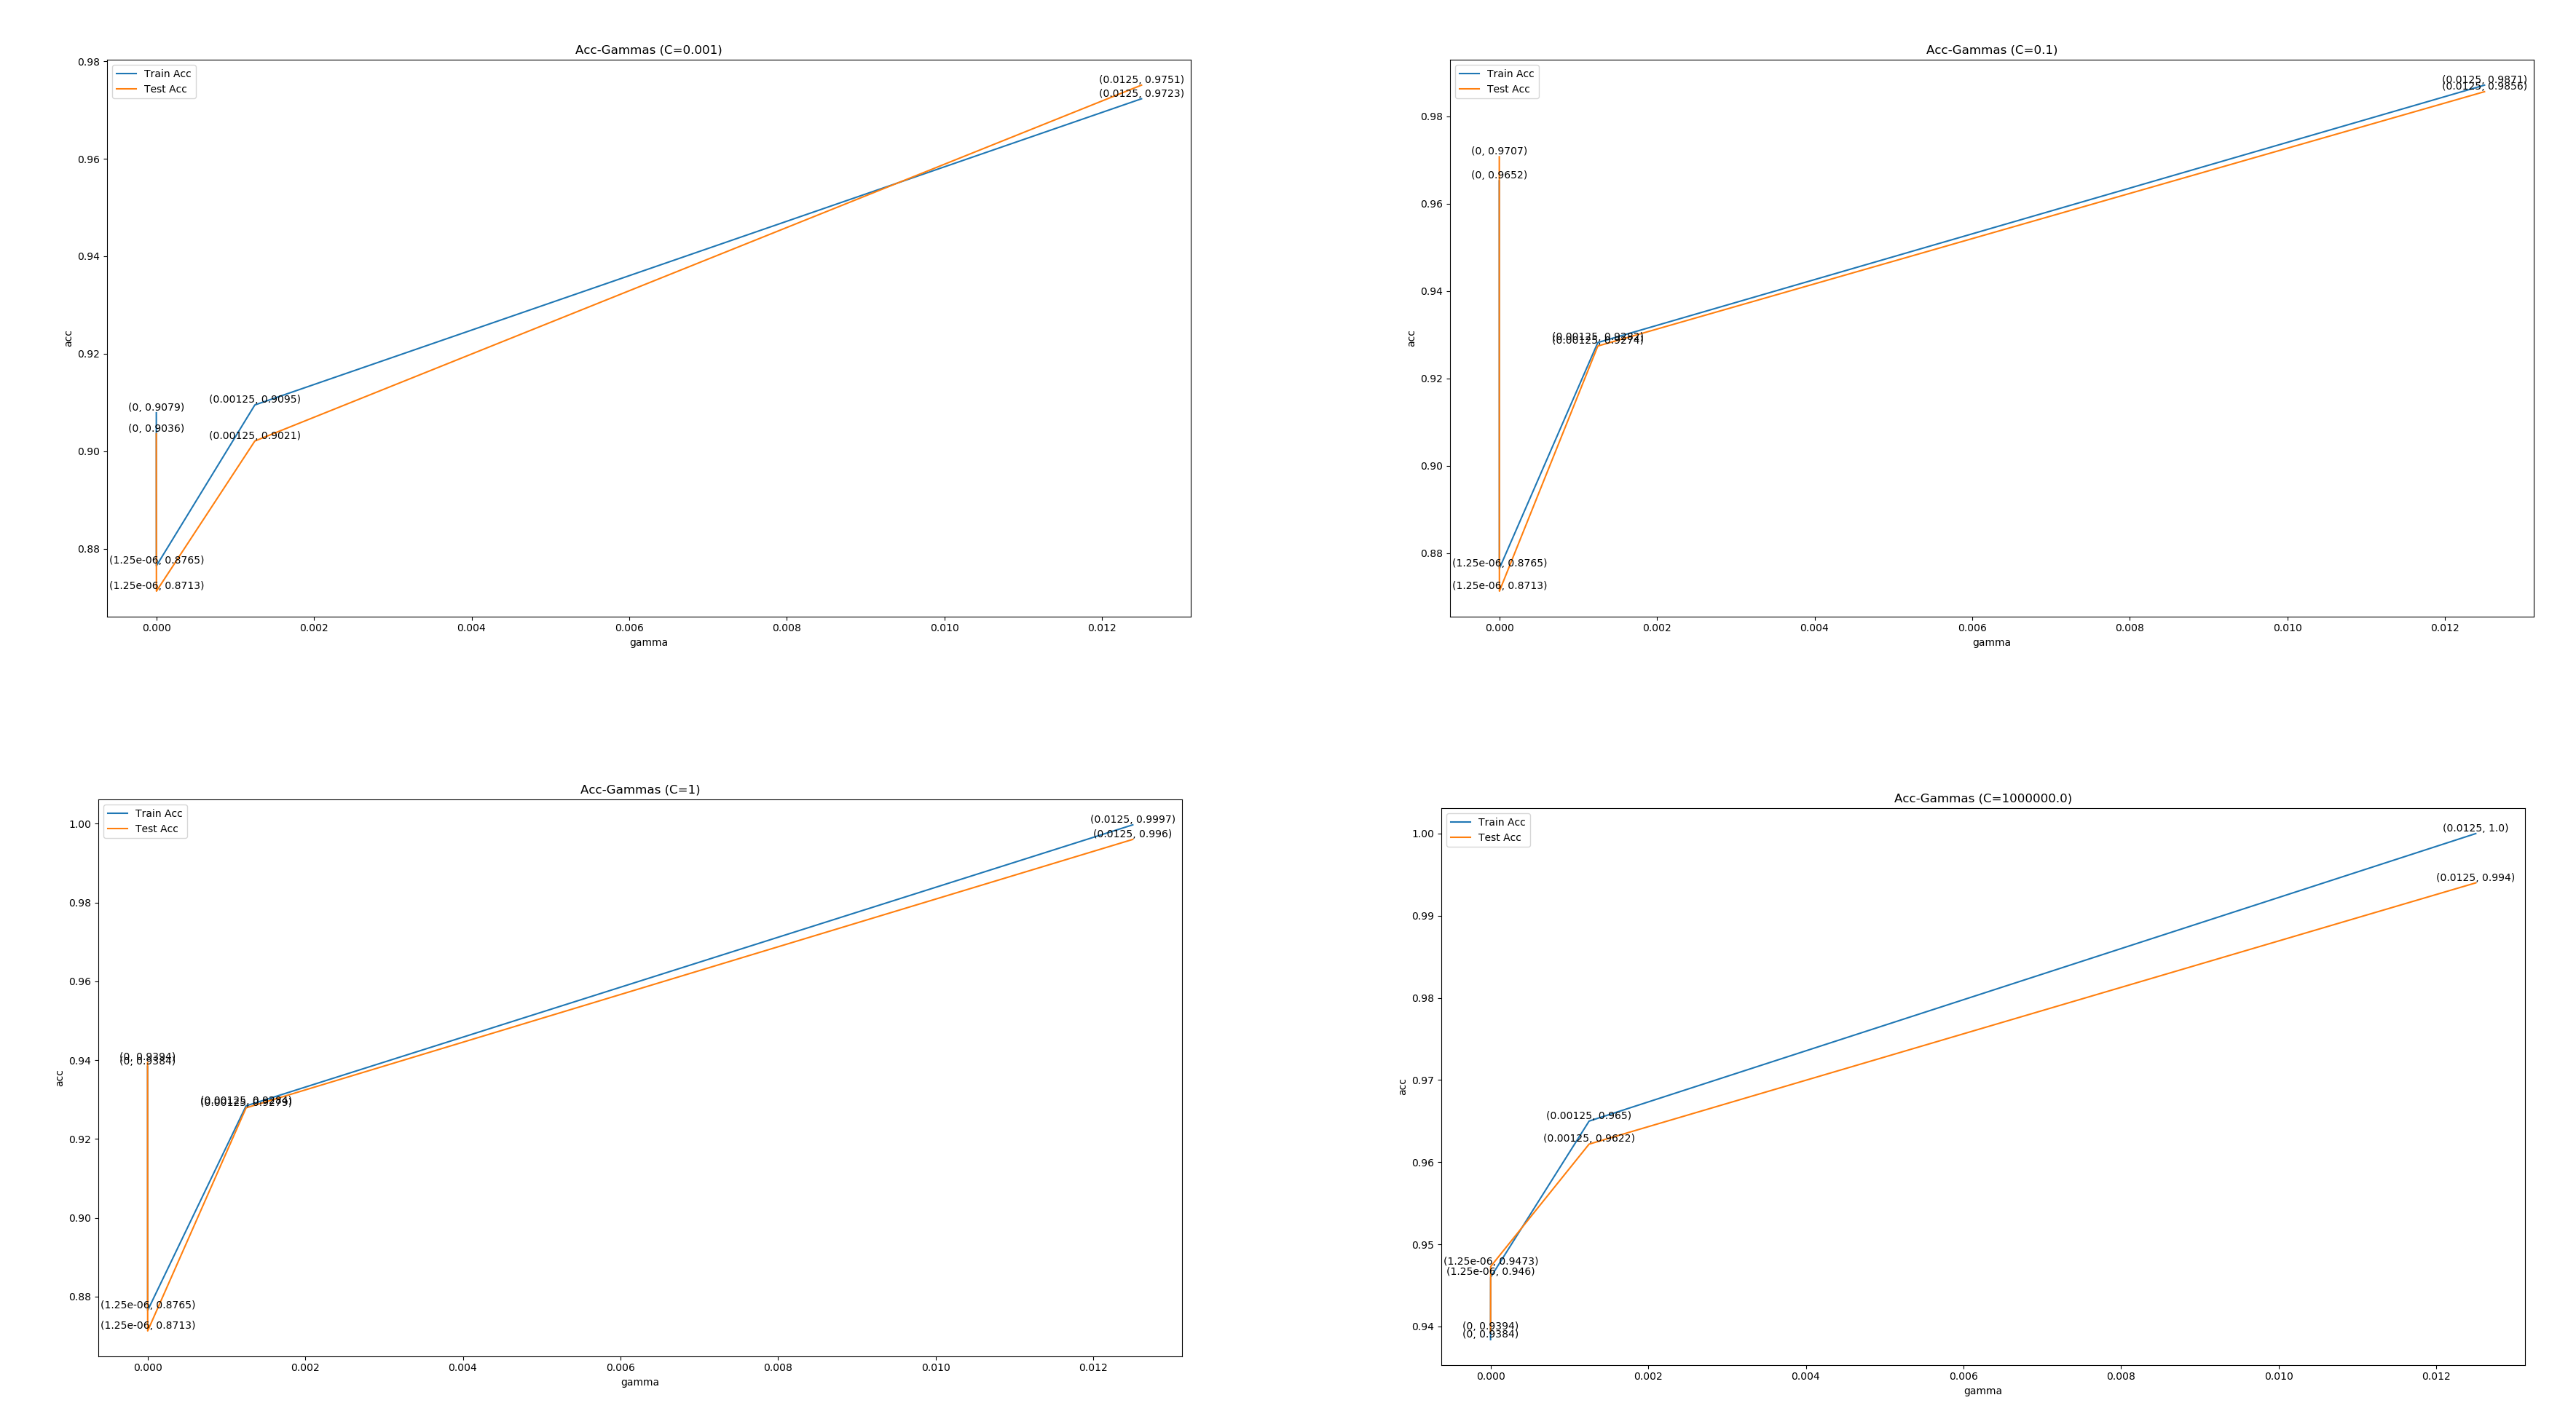
\includegraphics[width=\textwidth]{hw6.png}
    \caption{ Acc-gamma-C }
    \label{img1}
\end{figure}

\end{document}


\end{document}